\section{The LWE-based cryptosystem}

\subsection{Introduction}

The LWE-based cryptosystem is proved to be the most efficient lattice-based cryptosystem to date which is supported by a theoretical proof of security. The cryptosystem is shown to be secure based on the conjectured hardness of the \textbf{L}earning \textbf{W}ith \textbf{E}rrors problem (LWE), where the definition is shown below.

\begin{algorithm}
    \caption{Learning-With-Errors (LWE)}
    \begin{algorithmic}
        \State \textit{Parameters}: Integers $n, m, q \in \mathbb{Z}_{+}$ and a probability distribution $\chi : \mathbb{Z}_{q} \rightarrow[0,1]$.
        \State \textit{Instance}: A pair $(A, v)$ with $A \in \mathbb{Z}_{q}^{m \times n}$ and $v \in \mathbb{Z}_{q}^{m}$.
        \State \textit{Problem Task}: Decide if $v \in_{R} \mathbb{Z}_{q}^{m}$ was chosen uniformly at random or $v=A s+e$ was chosen with $s \in _R \mathbb{Z}_{q}^{n}$ and $e \in_{\chi} \mathbb{Z}_{q}^{m}$.
    \end{algorithmic}
\end{algorithm}

This problem can be equivalently described as a bounded distance decoding problem in $q$-ary lattices: Given $A \in_{R} \mathbb{Z}_{q}^{m \times n}$ and a vector $v \in \mathbb{Z}_{q}^{m},$ we need to distinguish between the case that $v$ is chosen uniformly from $\mathbb{Z}_{q}^{m}$ and the case in which $v$ is chosen by mangling each coordinate of a random point in $\Lambda_{q}\left(A^{T}\right)$ using $\chi^{m}.$

The LWE problem is believed to be very hard (for reasonable choices of parameters), with the best known algorithms running in exponential time in $n$. For a real $\alpha>0$ we let $\chi=\Psi_{\alpha}$ denote the distribution on $\mathbb{Z}_{q}$ obtained by sampling a normal variable with mean 0 and standard deviation $\alpha q / \sqrt{2 \pi}$ , rounding the result to the nearest integer and reducing it modulo $q$. Furthermore, we have the following theorem proven.

\begin{theorem}
    Assume access to an oracle that solves the LWE problem with a parameter choice $(n, m, q, \chi)$ such that $\chi=\Psi_{\alpha},\ \alpha q>\sqrt{n},$ a prime $q \leq \operatorname{poly}(n)$ and $m \leq \operatorname{poly}(n) .$ Then, there exists a quantum algorithm running in time poly $(n)$ for solving the SIVP$_{\gamma}$ and the decision variant of SVP$_{\gamma}$ for $\gamma=\tilde{\mathcal{O}}(n / \alpha)$ in any lattice of dimension $n$.\label{the1}
\end{theorem}

In other words, when we consider the security of lattice-based problems against quantum computers, any cryptosystem based on LWE is also secure against quantum computers. Moreover, it is very much possible that the proof for Theorem \ref{the1} may some day be dequantized, i.e. ported to a classical computational model, leading to a stronger security guarantee for LWE-based cryptosystems. Also, it has to be emphasized that the quantum arguments only show up in the LWE problem itself, and all of the cryptosystems based on it are entirely classical.

\subsection{Cryptosystem}

\subsubsection{Key Generation}

The cryptosystem is parameterized by integers $n, m, \ell, t, r, q,$ and a real $\alpha>0$. The parameter $n$ is in some sense the main security parameter, and it corresponds to the dimension of the lattices that show up in the worst-case connection. The generation pattern of both the public key and the private key is shown below.

\begin{algorithm}
    \caption{LWE-Key-Generation}
    \begin{algorithmic}[1]
        \Require $n, m, \ell, t, r, q \in \mathbb{Z}_{+}$ and $\alpha \in \mathbb{R}_{+}$
        \Ensure private key $S \in \mathbb{Z}_{q}^{n \times \ell}$ and public key $(A, P) \in \mathbb{Z}_{q}^{m \times n} \times \mathbb{Z}_{q}^{m \times \ell}$
        \State \textbf{choose} $S \in_{R} \mathbb{Z}_{q}^{n \times \ell}, A \in_{R} \mathbb{Z}_{q}^{m \times n}, E \in \Psi_{\alpha} \mathbb{Z}_{q}^{m \times \ell}$
        \State \textbf{set} $P :=A S+E$
        \State \Return $(S,(A, P))$
    \end{algorithmic}
\end{algorithm}

\subsubsection{Encryption}

To better understand the encryption algorithm, the following definition is needed.

\begin{definition}
    For integers $q, t \in \mathbb{Z}_{+},$ we define a function $\rho_{t}^{q} : \mathbb{Z}_{t} \rightarrow \mathbb{Z}_{q}$ by $$\rho_{t}^{q}(n) :=\left[\frac{n q}{t}\right].$$ We also write $\rho_{t}^{q}$ instead of $\left(\rho_{t}^{q}\right)^{\ell}$ when we apply this function to vectors in $\mathbb{Z}_{t}^{\ell}$.\label{def1}
\end{definition}

The encryption algorithm is shown below.

\begin{algorithm}
    \caption{LWE-Encryption}
    \begin{algorithmic}[1]
        \Require $n, m, \ell, t, r, q \in \mathbb{Z}_{+}, \alpha \in \mathbb{R}_{+},$ public key $(A, P) \in \mathbb{Z}_{q}^{m \times n} \times \mathbb{Z}_{q}^{m \times \ell},$ message $v \in \mathbb{Z}_{t}^{\ell}$
        \Ensure ciphertext $(u, c) \in \mathbb{Z}_{q}^{n} \times \mathbb{Z}_{q}^{\ell}$
        \State \textbf{choose} $a \in R[-r, r]^{m} \cap \mathbb{Z}^{m}$
        \State \textbf{set} $u :=A^{T} a$
        \State \textbf{set} $c :=P^{T} a+\rho_{t}^{q}(v)$
        \State \Return $(u,c)$
    \end{algorithmic}
\end{algorithm}

\subsubsection{Decryption}

The decryption algorithm is shown below. Also, to make the complete cryptosystem more intuitive, a schematic diagram is illustrated in Figure \ref{fig1} shown below as well.

\begin{algorithm}
    \caption{LWE-Decryption}
    \begin{algorithmic}[1]
        \Require ciphertext $(u, c) \in \mathbb{Z}_{q}^{n} \times \mathbb{Z}_{q}^{\ell},$ private key $S \in \mathbb{Z}_{q}^{n \times \ell}$
        \Ensure $v \in \mathbb{Z}_{t}^{\ell}$
        \State \Return $\rho_{q}^{t}\left(c-S^{T} u\right)$
    \end{algorithmic}
\end{algorithm}

\begin{figure}[htbp]
    \centering
    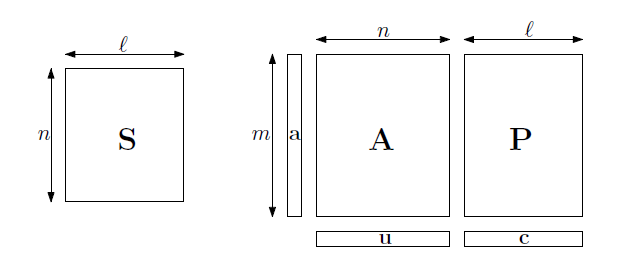
\includegraphics[height=5.0cm]{sgp1.PNG}
    \caption{Ingredients in the LWE-based cryptosystem.}
    \label{fig1}
\end{figure}

\subsection{Choosing Parameters}

The choice of parameters is meant to guarantee efficiency, a low probability of decryption errors, and security. In the following sections we will discuss how to choose the parameters in detail covering all these aspects.

\subsubsection{Efficiency}

The cryptosystem can be implemented efficiently since the operations only involve matrix addition and multiplication modulo a certain integer. Because of the features of computers, it is obvious to set $t=2^k$ to improve the running time. Also, the algorithms can be implemented with high level of parallelization, which is also easy to obtain.

\subsubsection{Decryption Errors}

Let $b :=E^{T} a$ and assume $\left|b_{i}\right|<\frac{q}{2 t}-\frac{1}{2} .$ We also set $w :=\rho_{t}^{q}(v),$ so we know
$$\left|\frac{q v_{i}}{t}-w_{i}\right| \leq \frac{1}{2} \Leftrightarrow\left|v_{i}-\frac{t w_{i}}{q}\right| \leq \frac{t}{2 q}$$

We now get 
$$\rho_{q}^{t}\left(b_{i}+\rho_{t}^{q}\left(v_{i}\right)\right)=\left[\frac{t \cdot\left(b_{i}+w_{i}\right)}{q}\right]$$

Therefore, we can calculate the estimate as
\begin{equation}
    \left|v_{i}-\frac{t \cdot\left(b_{i}+w_{i}\right)}{q}\right|=\left|v_{i}-\frac{t w}{q}\right|+\left|\frac{t b_{i}}{q}\right|<\frac{t}{2 q}+\left(\frac{1}{2}-\frac{t}{2 q}\right)=\frac{1}{2}\label{eq1}
\end{equation}

Thus, we can get 
\begin{align*}
    \rho_{q}^{t}\left(c-S^{T} u\right)&=\rho_{q}^{t}\left(P^{T} a+\rho_{t}^{q}(v)-S^{T} A^{T} a\right)\\
    &=\rho_{q}^{t}\left((A S+E)^{T} \cdot a+\rho_{t}^{q}(v)-S^{T} A^{T} a\right)\\
    &=\rho_{q}^{t}\left(E^{T} a+\rho_{t}^{q}(v)\right) \stackrel{(\ref{eq1})}{=} v
\end{align*}

Since $q$ is odd, if we assume $t$ to be even, we can conclude that
$$\left|b_{i}\right|<\frac{q}{2 t}-\frac{1}{2} \Leftrightarrow t\left|b_{i}\right|<\frac{q-t}{2} \Leftrightarrow t\left|b_{i}\right|<\frac{q}{2} \Leftrightarrow\left|b_{i}\right|<\frac{q}{2 t}$$

In other words, under this assumption, we can get
\begin{equation}
    \operatorname{Pr}\left[\rho_{q}^{t}\left(c-S^{T} u\right)=v\right] \geq \operatorname{Pr}\left[\forall i :\left|b_{i}\right|<\frac{q}{2 t}\right]\label{eq2}
\end{equation}

Now we analyze the behaviour of $b=E^{T} a$. Since each coordinate of $a$ is uniformly chosen from $[-r, r] \cap \mathbb{Z}$, we can get the variance of each coordinate
$$\operatorname{Var}\left(a_{i}\right)=\frac{1}{2 r+1} \cdot \sum_{k=-r} k^{2}=\frac{1}{2 r+1} \cdot \frac{r \cdot(r+1) \cdot(2 r+1)}{6}=\frac{r(r+1)}{3}$$

We denote by $X$ the random variable measuring $b_{i}$ and by $Z :=\frac{X-\mu(X)}{\sigma(X)}$ its normalization, such that $\operatorname{Pr}\left[z_{1} \leq Z \leq z_{2}\right]=\phi\left(z_{2}\right)-\phi\left(z_{1}\right) .$ Thus, we can calculate
    $$\sigma(X)^{2}=\operatorname{Var}\left(b_{i}\right)=\operatorname{Var}\left(\sum_{j=1}^{m} E_{j i} a_{j}\right)=\sum_{j=1}^{m} \operatorname{Var}\left(E_{j i}\right) \cdot \operatorname{Var}\left(a_{j}\right)=m \cdot \frac{\alpha^{2} q^{2}}{2 \pi} \cdot \frac{r(r+1)}{3}$$
and deduce an upper bound for the decryption error probability per letter:
\begin{align*}
    \operatorname{Pr}\left[|X| \geq \frac{q}{2 t}\right]&=\operatorname{Pr}\left[Z \geq \frac{q}{2 t \sigma(X)}\right]+\operatorname{Pr}\left[Z \leq \frac{-q}{2 t \sigma(X)}\right]\\
    &=1-\phi\left(\frac{q}{2 t \sigma(X)}\right)+\phi\left(\frac{-q}{2 t \sigma(X)}\right)\\
    &=2-2 \cdot \phi\left(\frac{q}{2 t \cdot \sigma(X)}\right)\\
    &=2 \cdot\left(1-\phi\left(\frac{1}{2 t \alpha} \cdot \sqrt{\frac{6 \pi}{r \cdot(r+1) \cdot m}}\right)\right)
\end{align*}

Plug into (\ref{eq2}), we can obtain
$$\operatorname{Pr}\left[\rho_{q}^{t}\left(c-S^{T} u\right) \neq v\right]<\operatorname{Pr}\left[\forall i :\left|b_{i}\right| \geq \frac{q}{2 t}\right]=1-\left(1-\operatorname{Pr}\left[\exists i :\left|b_{i}\right| \geq \frac{q}{2 t}\right]\right)^{\ell}$$

Then, the problem is deduced to mere arithmetics to adjust parameters accordingly to obtain low error margins. With some efforts, we can get the error-correcting codes to the plaintext to reduce the probability of decoding errors to a certain small value, which can be neglected.

\subsubsection{Security}

To meet the requirements of Theorem \ref{the1}, we choose $q$ to be prime and $\alpha q>\sqrt{n}$. This leaves us with a choice for $m$ and $\alpha$ where we will attempt to choose $\alpha$ as large as possible since it leads to harder lattice instances. Under these conditions, we may assume that the public keys are completely indistinguishable from pairs $(A, P)$ which is chosen uniformly at random. 

Despite all these theoretical results, we would like to describe an attack that is the best among all to break the cryptosystem. Assume that $(A, v)$ is an LWE-instance.

\begin{itemize}
    \item Choose a short vector $w \in \Lambda_{q}\left(A^{T}\right)^{*}$
    \item Calculate $\lambda :=\langle w, v\rangle$
    \item If $\lambda$ is close to an integer, we guess that $v=A s+e$ for some $e \in \Psi_{\alpha} \mathbb{Z}_{q}^{m}$
\end{itemize}

This method is based on the fact that 
$$\langle A s+e, w\rangle=\underbrace{\langle A s, w\rangle}_{\in \mathbb{Z}}+\langle e, w\rangle$$
and relies on $\langle e, w\rangle$ being very small. Fixing any vector $w$ and for $e \in \Psi_{\alpha} \mathbb{Z}_{q}^{m}$,
$$\operatorname{Var}(\langle e, w\rangle)=\operatorname{Var}\left(\sum_{i=1}^{m} e_{i} w_{i}\right)=\sum_{i=1}^{m} w_{i}^{2} \operatorname{Var}\left(e_{i}\right)=\|a\|^{2} \cdot \frac{\alpha^{2} q^{2}}{2 \pi}$$
yields a standard deviation of $\|w\| \cdot \frac{\alpha q}{\sqrt{2 \pi}}$ for this value. Since we want the above algorithm to fail, we choose
\begin{equation}
    \frac{\alpha q}{\sqrt{2 \pi}} \gg \frac{1}{\|w\|}\label{eq3}
\end{equation}

Based on the lattice reduction method, we have 
$$\Lambda_{q}\left(A^{T}\right)^{*}=q^{-1} \Lambda_{q}^{\perp}\left(A^{T}\right)$$
which result in
$$\|w\| \approx q^{-1} \cdot \min \left(q, 2^{\sqrt{4 n \log (q) \log (\delta)}}\right)$$

If right and left hand side of (\ref{eq3}) differ by a factor of $1.5,$ this brings the distribution of $\lambda$ mod $\mathbb{Z}$ into negligible statistical distance from the uniform distribution. Then, we get 
\begin{equation}
    \alpha \geq 1.5 \cdot \sqrt{2 \pi} \max \left(q^{-1}, 2^{-2} \sqrt{n \log (q) \log (\delta)}\right)\label{eq4}
\end{equation}

For a pair $(A, P) \in_{R} \mathbb{Z}_{q}^{m \times n} \times \mathbb{Z}_{q}^{m \times \ell}$ chosen uniformly at random and used as a public key for LWE-Encryption, we would like the ciphertext to be indistinguishable from a uniformly chosen vector. This would establish the cryptosystem extremely secure against chosen plaintext attacks.

\begin{theorem}
    Let $r<q$ be integers, $M \in R \mathbb{Z}_{q}^{n \times m}$ and $a \in R[-r, r]^{m} \cap \mathbb{Z}_{q}^{m} .$ Then, the statistical distance between the distribution of $M a$ and the uniform distribution on $\mathbb{Z}_{q}^{n}$ is bounded by $$\beta_{n, m}(q, r) :=\sqrt{\frac{(2 r+1)^{m}}{q^{n}}}$$\label{the2}
\end{theorem}

Choosing $M=\left(\begin{array}{c}{A^{T}} \\ {P T}\end{array}\right),$ Theorem \ref{the2} suggest we should choose parameters in such a way that $\beta_{n+\ell, m}(q, r)$ is negligible, which, in other words, $\beta_{n+\ell, m}(q, r)=2^{-100}$.

\subsubsection{Summary}

In this summary, we present some concrete choices of parameters, satisfying our aforementioned requirements. Thus, we expect them to deliver high levels of both security and efficiency. Equation (\ref{eq3}) result in the following choice:
$$m :=\frac{(n+\ell) \log (q)+200}{\log (2 r+1)}$$

Using an approximation parameter of $\delta=1.01$ corresponds to the most exact algorithm known, thus the estimate (\ref{eq4}) result in a choice of
$$\alpha :=4 \cdot \max \left\{q^{-1}, 2^{-2 \sqrt{n \log (q) \log (1.01)}}\right\}$$

We then can list some properties for the cryptosystem, which are quite intuitive and easy to observe, or otherwise ease to be derived from the above listed equations. The sizes are all in bits, and the logarithms are base 2.

\begin{itemize}
    \item Private key size: $n \ell \log q$
    \item Public key size: $m(n+\ell) \log q$
    \item Message size: $\ell \log t$
    \item Ciphertext size: $(n+\ell) \log q$
    \item Encryption blowup factor: $\left(1+\frac{n}{\ell}\right) \log q / \log t$
    \item Error probability per letter: $2 \cdot\left(1-\phi\left(\frac{1}{2 t \alpha} \cdot \sqrt{\frac{6 \pi}{r \cdot(r+1) \cdot m}}\right)\right)$
    \item Lattice dimension in attack: $\sqrt{n \log (q) / \log (\delta)}$
\end{itemize}

\begin{table}[!ht]
    \centering
    \begin{tabular}{|c||c|c|c|c|c|c|}
        \hline
        $n$ &136 &166& 192& 214& 233& 233\\\hline
        $l$ &136& 166& 192& 214& 233& 233\\\hline
        $m$ &2008& 1319& 1500& 1333& 1042& 4536\\\hline
        $q$ &2003& 4093& 8191& 16381& 32749& 32749\\\hline
        $r$ &1& 4& 5& 12& 59& 1\\\hline
        $t$ &2& 2&4 &4& 2 &40\\\hline
        $\alpha$ &0.0065& 0.0024& 0.0009959 &0.00045& 0.000217& 0.000217\\\hline
        Public key size in bits&$6\times 10^6$&$5.25\times 10^6$&$7.5\times 10^6$&$8\times 10^6$&$7.3\times 10^6$&$31.7\times 10^6$\\\hline
        Encryption blowup factor &21.9& 24& 13& 14& 30& 5.6\\\hline
        Error probability& 0.9\% &0.56\% &1\% &0.8\% &0.9\% &0.9\%\\\hline
        Lattice dimension in attack &322& 372& 417& 457 &493& 493\\\hline
    \end{tabular}
    \caption{Some possible choices of parameters using $\delta=1.01$.}
\end{table}